% (c) 2012-2014 Dimitrios Vrettos - d.vrettos@gmail.com
\chapter{Monomi}
\section{L'insieme dei monomi}

\begin{definizione}
Un'espressione letterale in cui numeri e lettere sono legati dalla sola moltiplicazione si chiama \emph{monomio}.
\end{definizione}

\begin{exrig}
 \begin{esempio}
L'espressione nelle due variabili~$a$ e~$b$, $E=5\cdot 2a^{2}\dfrac{3}{8}ab7b^{2}$
è un monomio perché numeri e lettere sono legate solo dalla moltiplicazione.
 \end{esempio}

 \begin{esempio}
L'espressione~$E=2a^{2}-ab^{2}$ non è un monomio poiché compare anche il segno di sottrazione.
 \end{esempio}
\end{exrig}

\ovalbox{\risolvi \ref{ese:10.1}}

\osservazione
Gli elementi di un monomio sono \emph{fattori}, perché sono termini
di una moltiplicazione ma possono comparire anche \emph{potenze},
infatti la potenza è una moltiplicazione di fattori uguali. Non
possono invece comparire esponenti negativi o frazionari. In un monomio
gli esponenti delle variabili devono essere numeri naturali.

\begin{definizione}
Un monomio si dice \emph{ridotto in forma normale} quando è scritto come prodotto di un solo fattore
numerico e di potenze letterali con basi diverse.
\end{definizione}

\begin{exrig}
 \begin{esempio}
Il monomio~$E=5\cdot 2a^{2}\dfrac{3}{8}ab7b^{2}$ non è scritto in
forma normale: tra i suoi fattori vi sono numeri diversi e le potenze
letterali hanno basi ripetute, la~$a$ e la~$b$ compaiono due volte ciascuna.

Moltiplichiamo tra loro i fattori numerici e otteniamo~$\dfrac{105}{4}$; eseguiamo il prodotto di potenze con la stessa base otteniamo
$a^{3}b^{3}$. Il monomio in forma normale è~$E=\dfrac{105}{4}a^{3}b^{3}$.
 \end{esempio}
\end{exrig}

\begin{procedura}
 Ridurre in forma normale un monomio:
 \begin{enumeratea}
 \item moltiplicare tra loro i fattori numerici;
 \item moltiplicare le potenze con la stessa base.
 \end{enumeratea}
\end{procedura}

\ovalbox{\risolvi \ref{ese:10.2}}

\begin{definizione}
La parte numerica del monomio ridotto a forma normale si chiama \emph{coefficiente} e
il complesso delle lettere ne costituisce la \emph{parte letterale}.
\end{definizione}

\begin{exrig}
 \begin{esempio}
 Nella tabella seguente sono segnati alcuni monomi con i rispettivi coefficienti e parti letterali.
\begin{center}
 \begin{tabular}{lcccc}
 \toprule
 monomio & $-{\dfrac{1}{2}}abc$ & $3x^{3}y^{5}$ & $a^{5}b^{7}$ & $-k^{2}$\\
coefficiente & $-{\dfrac{1}{2}}$ & $3$ & $1$ & $-1$ \\
parte letterale & $abc$ & $x^{3}y^{5}$ & $a^{5}b^{7}$ & $k^{2}$ \\
 \bottomrule
\end{tabular}
\end{center}
 \end{esempio}
\end{exrig}

\begin{definizione}
Se il coefficiente del monomio è zero il \emph{monomio} si dice \emph{nullo}.
\end{definizione}

\begin{exrig}
 \begin{esempio}
L'espressione letterale~$\frac{3}{5}a^{3}bc^{2}$ è un monomio;
il numero~$\frac{3}{5}$ e le lettere~$a^{3}$, $b$, $c^{2}$ sono legate
dall'operazione di moltiplicazione; il suo coefficiente è il numero~$\frac{3}{5}$ e la parte letterale è~$a^{3}bc^{2}$.
 \end{esempio}

 \begin{esempio}
 Controesempi:

 \begin{enumeratea}
 \item l'espressione letterale~$\frac{3}{5}a^{3}+bc^{2}$
 non è un monomio dal momento che numeri e lettere sono legati, oltre
che dalla moltiplicazione, anche dall'addizione;
\item l'espressione letterale~$\frac{3}{5}a^{-3}bc^{2}$
non è un monomio in quanto la potenza con esponente negativo
rappresenta una divisione, infatti~$a^{-3}=\frac{1}{a^{3}}$.
\end{enumeratea}
 \end{esempio}
\end{exrig}

\begin{definizione}
 Due o più monomi che hanno parte letterale identica si dicono \emph{simili}.
\end{definizione}

\begin{exrig}
 \begin{esempio}
Il monomio~$\frac{3}{5}a^{3}bc^{2}$ è simile
a~$68a^{3}bc^{2}$ e anche a~$-0,5a^{3}bc^{2}$, ma non è simile
a~$\frac{3}{5}a^{2}bc^{3}$. L'ultimo monomio ha le
stesse lettere degli altri ma sono elevate ad esponenti diversi.
 \end{esempio}
\end{exrig}

\osservazione Il monomio nullo si considera simile a qualunque altro monomio.

\begin{definizione}
Due monomi simili che hanno coefficiente opposto si dicono \emph{monomi opposti}.
\end{definizione}

%\begin{exrig}
 \begin{esempio}
I monomi~$\frac{3}{5}a^{3}bc^{2}$ e~$-{\frac{3}{5}}a^{3}bc^{2}$ sono opposti, infatti sono simili e hanno
coefficienti opposti.
\end{esempio}

\begin{esempio}
Non sono opposti~$\frac{3}{5}a^{3}bc^{2}$ e~$-7a^{3}bc^{2}$ ma semplicemente simili. I loro coefficienti hanno segno diverso, ma
non sono numeri opposti.
\end{esempio}
%\end{exrig}

%\ovalbox{\risolvi \ref{ese:10.3}}

\begin{definizione}
Quando il monomio è ridotto a forma normale, l'esponente di una sua variabile ci indica il
\emph{grado} del monomio \emph{rispetto a quella variabile}.

Il \emph{grado complessivo} di un monomio è la somma degli esponenti della parte letterale.
\end{definizione}

\begin{exrig}
 \begin{esempio}
Il monomio~$\frac{3}{5}a^{3}bc^{2}$ ha grado complessivo~6,
ottenuto sommando gli esponenti della sua parte letterale~$(3+1+2=6)$.
Rispetto alla variabile~$a$ è di terzo grado, rispetto alla
variabile~$b$ è di primo grado, rispetto alla variabile
$c$ è di secondo grado.
 \end{esempio}
\end{exrig}

Abbiamo detto che gli esponenti della parte letterale del monomio sono
numeri naturali, dunque possiamo anche avere una o più variabili
elevate ad esponente~0. Cosa succede allora nel monomio?

Consideriamo il monomio~$56a^{3}b^{0}c^{2}$, sappiamo che qualunque
numero diverso da zero elevato a zero è uguale a~1, quindi possiamo
sostituire la variabile~$b$ che ha esponente~0 con~1 e
otteniamo~$56a^{3}\cdot 1\cdot c^{2}=56a^{3}c^{2}$. Se in un monomio ogni
variabile ha esponente~0, il monomio rimane solamente con il suo
coefficiente numerico: per esempio~$-3a^{0}x^{0}=-3\cdot 1\cdot 1=-3$.

\osservazione Esistono \emph{monomi di grado~0}; essi presentano solo il
coefficiente e pertanto \emph{sono} equiparabili ai \emph{numeri razionali}.

\section{Valore di un monomio}

Poiché il monomio è un'espressione letterale,
possiamo calcolarne il valore quando alle sue variabili sostituiamo dei numeri.

\begin{exrig}
 \begin{esempio}
 Calcola il valore del monomio~$3x^{4}y^{5}z$ per i valori~$x=-3$, $y=5$ e~$z=0$.

Sostituendo i valori assegnati otteniamo~$3\cdot (-3)^{4}\cdot 5^{5}\cdot 0=0$ essendo uno dei fattori nullo.
 \end{esempio}
\end{exrig}

\osservazione Il valore di un monomio è nullo quando almeno una delle sue variabili
assume il valore~0.

Molte formule di geometria sono scritte sotto forma di monomi: area del
triangolo~$\frac{1}{2}bh$, area del quadrato~$l^{2}$,
perimetro del quadrato~$4l$, area del rettangolo~$bh$, volume del cubo~$l^{3}$, ecc.
Esse acquistano un valore quando alle lettere sostituiamo
i numeri che rappresentano le misure della figura considerata.

\ovalbox{\risolvii \ref{ese:10.3}, \ref{ese:10.4}, \ref{ese:10.5}, \ref{ese:10.6}, \ref{ese:10.7}, \ref{ese:10.8}, \ref{ese:10.9}, \ref{ese:10.10}, \ref{ese:10.11}}

\section{Moltiplicazione di due monomi}

Ci proponiamo ora di introdurre nell'insieme dei monomi
le operazioni di addizione, sottrazione, moltiplicazione, potenza e
divisione.

Ricordiamo che definire un'operazione all'interno di un insieme
significa stabilire una legge che associa a due elementi
dell'insieme un altro elemento
dell'insieme stesso.

La moltiplicazione di due monomi si indica con lo stesso simbolo della
moltiplicazione tra numeri; i suoi termini si chiamano \emph{fattori} e il
risultato si chiama \emph{prodotto}, proprio come negli insiemi numerici.

\begin{definizione}
 Il prodotto di due monomi è il monomio avente
per coefficiente il prodotto dei coefficienti e per parte letterale il
prodotto delle parti letterali dei monomi fattori.
\end{definizione}

\begin{exrig}
 \begin{esempio}
Assegnati i monomi~$m_{1}=-4x^{2}yz^{3}$ e~$m_{2}=\dfrac{5}{6}x^{3}z^{6}$,
il monomio prodotto è
\[m_{3}=\bigg(-4\cdot {\frac{5}{6}}\bigg)\big(x^{2}\cdot x^{3}\big)\cdot y\cdot \big(z^{3}\cdot z^{6}\big)=-\frac{10}{3}x^{5}yz^{9}.\]
 \end{esempio}
\end{exrig}


\begin{procedura}[per moltiplicare due monomi]
La moltiplicazione tra monomi si effettua moltiplicando prima i
coefficienti numerici e dopo le parti letterali:

\begin{enumeratea}
 \item nella moltiplicazione tra i coefficienti usiamo le regole note della
moltiplicazione tra numeri razionali;
 \item nella moltiplicazione tra le parti letterali applichiamo la regola
del prodotto di potenze con la stessa base.
\end{enumeratea}
\end{procedura}

\subsection{Proprietà della moltiplicazione}

\begin{enumeratea}
\item commutativa:~$m_{{1}}\cdot m_{2}=m_{2}\cdot m_{{1}}$;
\item associativa:~$m_{{1}}\cdot m_{2}\cdot m_{3}=(m_{{1}}\cdot m_{2})\cdot m_{3}=m_{{1}}\cdot (m_{2}\cdot m_{3})$;
\item 1 è l'elemento neutro:~$1\cdot m=m\cdot 1=m$;
\item se uno dei fattori è uguale a~0 il prodotto è~0, cioè~$0\cdot m=m\cdot 0=0$.
\end{enumeratea}

\ovalbox{\risolvii \ref{ese:10.12}, \ref{ese:10.13}, \ref{ese:10.14}, \ref{ese:10.15}}

\section{Potenza di un monomio}

Ricordiamo che tra i numeri l'operazione di elevamento a
potenza ha un solo termine, la base, sulla quale si agisce a seconda
dell'esponente.

\[\text{Potenza }=\text{ base }^\text{ esponente}= \underbrace{(\text{ base }\cdot \text{ base }\cdot\text{ base }\cdot\ldots\cdot \text{ base })}_{\text{tanti fattori quanti ne indica l'esponente}}.\]

Analogamente viene indicata la potenza di un monomio: la base è un
monomio e l'esponente è un numero naturale.

\begin{definizione}
La \emph{potenza di un monomio} è un monomio
avente per coefficiente la potenza del coefficiente e per parte
letterale la potenza della parte letterale.
\end{definizione}

\begin{exrig}
 \begin{esempio}
Calcoliamo il quadrato e il cubo del monomio~$m_{1}=-{\dfrac{1}{2}}a^{2}b$.
\[\text{elevo al quadrato}\quad\Rightarrow\quad\bigg(-{\frac{1}{2}}a^{2}b\bigg)^{2}
=\bigg(-{\frac{1}{2}}\bigg)^{2}\cdot\big(a^{2}\big)^{2}\cdot (b)^{2}=\frac{1}{4}a^{4}b^{2}.\]

\[\text{elevo al cubo}\quad\Rightarrow\quad\bigg(-{\frac{1}{2}}a^{2}b\bigg)^{3}
=\bigg(-{\frac{1}{2}}\bigg)^{3}\cdot\big(a^{2}\big)^{3}\cdot (b)^{3}
=-{\frac{1}{8}}a^{6}b^{3}.\]
 \end{esempio}

 \begin{esempio}
Calcoliamo il quadrato e il cubo del monomio~$m_{2}=5a^{3}b^{2}c^{2}$.
\[\text{elevo al quadrato}\quad\Rightarrow\quad\big(5a^{3}b^{2}c^{2}\big)^{2}
=\big(5\big)^{2}\cdot \big(a^{3}\big)^{2}\cdot\big(b^{2}\big)^{2}\cdot \big(c^{2}\big)^{2}
=25a^{6}b^{4}c^{4}.\]

\[\text{elevo al cubo}\quad\Rightarrow\quad\big(5a^{3}b^{2}c^{2}\big)^{3}
=\big(5\big)^{3}\cdot \big(a^{3}\big)^{3}\cdot\big(b^{2}\big)^{3}\cdot \big(c^{2}\big)^{3}
=125a^{9}b^{6}c^{6}.\]
 \end{esempio}
\end{exrig}

\begin{procedura}
Eseguire l'elevazione a potenza di un monomio:

\begin{enumeratea}
 \item applichiamo la proprietà relativa alla potenza di un prodotto,
eseguiamo cioè la potenza di ogni singolo fattore del monomio;
 \item applichiamo la proprietà relativa alla potenza di potenza,
moltiplicando l'esponente della variabile per l'esponente delle potenza.
\end{enumeratea}
\end{procedura}

\ovalbox{\risolvii \ref{ese:10.16}, \ref{ese:10.17}, \ref{ese:10.18}, \ref{ese:10.19}}

\section{Divisione di due monomi}

Premessa: ricordiamo che assegnati due numeri razionali~$d_{1}$
e~$d_{2}$ con~$d_{2}\neq~0$, eseguire la
divisione~$d_{1}:d_{2}$ significa determinare il numero~$q$
che moltiplicato per~$d_{2}$ dà~$d_{1}$.
Nell'insieme~$\insQ$ la condizione~$d_{2}\neq~0$ è sufficiente per
affermare che~$q$ esiste ed è un numero razionale.

\begin{definizione}
Assegnati due monomi~$m_{1}$ e~$m_{2}$ con~$m_{2}$ diverso dal monomio nullo, se
è possibile determinare il monomio~$q$ tale che~$m_{1} = q\cdot m_{2}$, si dice che~$m_{1}$ è
divisibile per~$m_{2}$ e~$q$ è il monomio \emph{quoziente}.
\end{definizione}

\begin{exrig}
 \begin{esempio}
$(36x^{5}y^{2}):(-18x^{3}y)$.

Per quanto detto sopra, vogliamo trovare, se esiste, il monomio~$q$ tale
che~$(36x^{5}y^{2})=q\cdot (-18x^{3}y)$
e ripensando alla moltiplicazione di monomi possiamo dire
che~$q=-2x^{2}y$. Infatti~$(-2x^{2}y)\cdot(-18x^{3}y)=(36x^{5}y^{2})$. Il monomio~$-2x^{2}y$
è quindi il quoziente della divisione assegnata.
 \end{esempio}
\end{exrig}

\begin{procedura}[Calcolare il quoziente di due monomi]
Il quoziente di due monomi è così composto:
\begin{enumeratea}
 \item il coefficiente è il quoziente dei coefficienti dei monomi dati;
 \item la parte letterale ha gli esponenti ottenuti sottraendo gli esponenti
delle stesse variabili;
 \item se la potenza di alcune lettere risulta negativa il risultato della
divisione non è un monomio.
\end{enumeratea}
\end{procedura}
\pagebreak
\begin{exrig}
 \begin{esempio}
$\bigg(\dfrac{7}{2}a^{3}x^{{4}}y^{2}\bigg):\bigg(-{\dfrac{21}{8}}ax^{2}y\bigg)$.

Seguiamo i passi descritti sopra
\[\bigg(\frac{7}{2}a^{3}x^{{4}}y^{2}\bigg):\bigg(-{\frac{21}{8}}ax^{2}y\bigg)=\frac{7}{2}\cdot%
\bigg(-{\frac{8}{21}}\bigg)a^{3-1}x^{4-2}y^{2-1}=-{\frac{4}{3}}a^{2}x^{2}y.\]

Nell'eseguire la divisione non abbiamo tenuto conto
della condizione che il divisore deve essere diverso dal monomio nullo;
questa condizione ci obbliga a stabilire per la divisione le Condizioni
di Esistenza,~$\CE:a\neq0\text{ e }x\neq~0\text{ e }y\neq~0$.
 \end{esempio}

 \begin{esempio}
$\bigg(\dfrac{9}{20}a^{2}b^{4}\bigg):\bigg(-{\dfrac{1}{8}}a^{5}b^{2}\bigg)$.

La~$\CE a\neq~0\text{ e }b\neq~0$, il quoziente è
\[\bigg(\frac{9}{20}a^{2}b^{4}\bigg):\bigg(-{\frac{1}{8}}a^{5}b^{2}\bigg)=%
\bigg(\frac{9}{20}\bigg)\cdot(-8)a^{2-5}b^{4-2}=-{\frac{18}{5}}a^{-3}b^{2}.\]

Osserviamo che il quoziente ottenuto non è un monomio perché
l'esponente della variabile~$a$ è negativo. Il
risultato è un'espressione frazionaria o fratta.
 \end{esempio}
\end{exrig}

In conclusione, l'operazione di divisione tra due monomi
ha come risultato un monomio se ogni variabile del dividendo ha
esponente maggiore o uguale all'esponente con cui
compare nel divisore.


\vspazio\ovalbox{\risolvii \ref{ese:10.20}, \ref{ese:10.21}, \ref{ese:10.22}}

\section{Addizione di due monomi}

L'addizione di due monomi si indica con lo stesso
simbolo dell'addizione tra numeri; i suoi termini si
chiamano \emph{addendi} e il risultato si chiama \emph{somma}.

\subsection{Addizione di due monomi simili}

La somma di due monomi simili è un monomio simile agli addendi e
avente come coefficiente la somma dei coefficienti.

\begin{exrig}
 \begin{esempio}
Calcoliamo~$3x^{3}+(-6x^{3})$.

I due addendi sono monomi simili dunque la somma è ancora un monomio
ed è simile ai singoli addendi. Precisamente
$3x^{3}+(-6x^{3})=(3+(-6))x^{3}=-3x^{3}$.

Osserva che la somma di monomi simili si riduce alla somma algebrica di numeri.
 \end{esempio}
\end{exrig}

\ovalbox{\risolvi \ref{ese:10.23}}

\subsubsection{Proprietà dell'addizione}

\begin{enumeratea}
 \item commutativa:~$m_{{1}}+m_{2}=m_{2}+m_{{1}}$;
 \item associativa:~$m_{{1}}+m_{2}+m_{3}=(m_{{1}}+m_{2})+m_{3}=m_{{1}}+(m_{2}+m_{3})$;
 \item 0 è l'elemento neutro:~$0+m=m+0=m$;
 \item per ogni monomio m esiste il monomio \emph{opposto}, cioè un
 monomio~$m\Ast$ tale che
 \[m + m\Ast = m\Ast +m=0.\]
\end{enumeratea}

L'ultima proprietà enunciata ci permette di definire
nell'insieme dei monomi simili anche la sottrazione di
monomi. Essa si indica con lo stesso segno della sottrazione tra numeri
e il suo risultato si chiama \emph{differenza}.

\osservazione Per sottrarre due monomi simili si aggiunge al primo
l'opposto del secondo.

\begin{exrig}
 \begin{esempio}
Assegnati~$m_{{1}}=\dfrac{1}{2}a^{2}b$, $m_{2}=-\text{5a}^{2}b$ determina~$m_{1} - m_{2}$.

L'operazione richiesta
$\dfrac{1}{2}a^{2}b-(-5a^{2}b)$ diventa
$\dfrac{1}{2}a^{2}b+5a^{2}b=\dfrac{11}{2}a^{2}b$.
 \end{esempio}
\end{exrig}

Sulla base di quanto detto, possiamo unificare le due operazioni di
addizione e sottrazione di monomi simili in un'unica
operazione che chiamiamo \emph{somma algebrica di monomi}.

\osservazione La somma algebrica di due monomi simili è un monomio simile agli
addendi avente per coefficiente la somma algebrica dei coefficienti.

\begin{exrig}
 \begin{esempio}
Determiniamo la somma~$\dfrac{3}{5}x^{{4}}-\dfrac{1}{3}x^{{4}}+x^{{4}}+\dfrac{4}{5}x^{{4}}-2x^{{4}}-\dfrac{1}{2}x^{{4}}$.

Osserviamo che tutti gli addendi sono tra loro simili dunque:
\[\frac{3}{5}x^{{4}}-\frac{1}{3}x^{{4}}+x^{{4}}+\frac{4}{5}x^{{4}}-2x^{{4}}-\frac{1}{2}x^{{4}}=\left(\frac{3}{5}-\frac{1}{3}+1+\frac{4}{5}-2-\frac{1}{2}\right)x^{{4}}=-{\frac{13}{30}}x^{{4}}.\]
\end{esempio}
\end{exrig}
%\newpage
\subsection{Addizione di monomi non simili}

Analizziamo il caso della seguente
addizione:~$7a^{3}b^{2}-5a^{2}b^{3}+a^{3}b^{2}$. Si vuole determinare
la somma. I monomi addendi non sono tutti tra loro simili; lo sono
però il primo e il terzo.

Le proprietà associativa e commutativa ci consentono di riscrivere
l'addizione precedente
``avvicinando'' i monomi simili e
sostituendo ad essi la loro
somma:
\[7a^{3}b^{2}-5a^{2}b^{3}+a^{3}b^{2}=(7a^{3}b^{2}+a^{3}b^{2})-5a^{2}b^{3}=8a^{3}b^{2}-5a^{2}b^{3}.\]

L'espressione così ottenuta è la somma richiesta.

%\vspazio\ovalbox{\risolvi \ref{ese:10.24}}\vspazio

Il procedimento che abbiamo seguito per determinare il risultato
dell'addizione assegnata viene chiamato
\emph{riduzione dei termini simili}.

In conclusione, l'operazione di addizione tra monomi ha
come risultato un monomio solo se gli addendi sono monomi simili; in
caso contrario la somma viene effettuata riducendo i monomi simili e
lasciando indicata l'addizione tra gli altri monomi.
\pagebreak
\begin{exrig}
 \begin{esempio}
Calcola la seguente somma:~$3a-7a+2a+a$.

Il risultato è un monomio poiché gli addendi sono monomi
simili, e vale $-a$.
 \end{esempio}

 \begin{esempio}
Calcola la seguente somma:
$\dfrac{1}{2}a^{3}+b-\dfrac{3}{4}a^{3}-\dfrac{6}{5}b$.

Il risultato non è un monomio poiché gli addendi non sono
monomi simili: $-{\dfrac{1}{4}}a^{3}-\dfrac{1}{5}b$.
 \end{esempio}
\end{exrig}

\ovalbox{\risolvii \ref{ese:10.24}, \ref{ese:10.25}, \ref{ese:10.26}, \ref{ese:10.27}, \ref{ese:10.28}, \ref{ese:10.29}, \ref{ese:10.30}, \ref{ese:10.31}}

\section{Espressioni con i monomi}
Consideriamo l'espressione letterale
$E=\left(-{\frac{1}{2}}a^{2}b\right)^{3}:(a^{5}b)+(-2ab)\cdot\left(\frac{1}{2}b+b\right)+5ab^{2}$.

Vediamo che è in due variabili, le variabili sono infatti~$a$ e~$b$. Inoltre, i termini delle operazioni che vi compaiono sono monomi.

Se volessimo calcolare il valore di~$E$ per~$a = 10$ e $b = -2$ dovremmo
sostituire nell'espressione tali valori e risolvere
l'espressione numerica che ne risulta. Inoltre se
dovessimo calcolare il valore di~$E$ per altre coppie dovremmo ogni volta
applicare questo procedimento.

Dal momento che abbiamo studiato come eseguire le operazioni razionali
con i monomi, prima di sostituire i numeri alle lettere, applichiamo le
regole del calcolo letterale in modo da ridurre~$E$, se possibile,
in un'espressione più semplice.

Prima di procedere, essendovi una divisione, poniamo innanzi tutto
la~$\CE a \neq~0$ e~$b \neq~0$ ed eseguiamo rispettando la precedenza
delle operazioni come facciamo nelle espressioni numeriche.
%\newpage
\begin{exrig}
 \begin{esempio}
Calcola $\bigg(-{\dfrac{1}{2}}a^{2}b\bigg)^{3}:(a^{5}b)+(-2ab)\cdot\bigg(\dfrac{1}{2}b+b\bigg)+5ab^{2}$ per $a=10$ e $b=-2$.
 \begin{align*}
 &\text{sviluppiamo per prima il cubo} && = \bigg(-{\frac{1}{8}}a^{6}b^{3}:a^{5}b\bigg)+(-2ab)\cdot{\frac{3}{2}}b+5ab^{2} \\
 &\text{eseguiamo divisione e moltiplicazione} && = -{\frac{1}{8}}ab^{2}-3ab^{2}+5ab^{2}\\
 &\text{sommiamo i monomi simili} && = \frac{15}{8}ab^{2}.
 \end{align*}
 Ora è più semplice calcolarne il valore per~$a=10$ e~$b=-2$: si
 ha~$=\frac{15}{8}\cdot 10\cdot(-2)^{2}=\frac{15}{8}\cdot 10\cdot 4=75$.
 \end{esempio}

 \begin{esempio}
Riduci l'espressione $\bigg(\dfrac{2}{3}ab^{2}c\bigg)^{2}:\big(-3ab^{3}\big)-\dfrac{2}{9}abc^{2}$.
 \begin{align*}
 &\text{Sviluppiamo le potenze} && = \frac{4}{9}a^{2}b^{4}c^{2}:\big(-3ab^{3}\big)-\frac{2}{9}abc^{2}\\
 &\text{eseguiamo la divisione e moltiplichiamo le frazioni} && = -{\frac{4}{27}}abc^{2}-\frac{2}{9}abc^{2}\\
 &\text{sommiamo i monomi simili} && = \frac{-4-6}{27}abc^{2}\\
 &\text{il risultato è} && = -{\frac{10}{27}}abc^{2}.
 \end{align*}
 \end{esempio}

 \begin{esempio}
Riduci l'espressione $\Bigg[\bigg(-{\dfrac{14}{16}}x^{2}y^{2}\bigg):\bigg(-{\dfrac{14}{4}}xy\bigg)\Bigg]^{3}+\dfrac{1}{2}xy\cdot{\dfrac{1}{4}}x^{2}y^{2}$.
 \begin{align*}
 &\text{Eseguiamo la divisione tra le parentesi quadre} && = \bigg[+{\frac{14}{16}}\cdot{\frac{4}{14}}xy\bigg]^{3}+\frac{1}{2}xy\cdot {\frac{1}{4}}x^{2}y^{2}\\
 &\text{eseguiamo la moltiplicazione tra le frazioni} && = \bigg[\frac{1}{4}xy\bigg]^{3}+\frac{1}{2}xy\cdot{\frac{1}{4}}x^{2}y^{2}\\
 &\text{sviluppiamo il cubo} && = \frac{1}{64}x^{3}y^{3}+\frac{1}{2}xy\cdot {\frac{1}{4}}x^{2}y^{2}\\
 &\text{moltiplichiamo i due monomi} && = \frac{1}{64}x^{3}y^{3}+\frac{1}{8}x^{3}y^{3}\\
 &\text{sommiamo i monomi simili} && = \frac{1+8}{64}x^{3}y^{3}\\
 &\text{il risultato è} && = \frac{9}{64}x^{3}y^{3}.
\end{align*}
 \end{esempio}
\end{exrig}

\ovalbox{\risolvii \ref{ese:10.32}, \ref{ese:10.33}, \ref{ese:10.34}, \ref{ese:10.35}, \ref{ese:10.36}, \ref{ese:10.37}, \ref{ese:10.38}, \ref{ese:10.39}, \ref{ese:10.40}, \ref{ese:10.41},}

\vspazio\ovalbox{\ref{ese:10.42}, \ref{ese:10.43}}

\section{Massimo Comune Divisore e minimo comune multiplo tra monomi}
\subsection{Massimo Comune Divisore}

Il calcolo del minimo comune multiplo e del Massimo Comune Divisore,
studiato per i numeri, si estende anche ai monomi. Premettiamo intanto
le seguenti definizioni.

\begin{definizione}
 Un monomio~$A$ si dice \emph{multiplo} di un monomio~$B$ se esiste un
monomio~$C$ per il quale si ha~$A=B\cdot C$; in questo caso diremo anche che~$B$
è \emph{divisore} del monomio~$A$.
\end{definizione}

\begin{definizione}
 Il \emph{massimo comune divisore} ($\mcd$) tra due o più monomi è il
monomio che, tra tutti i divisori comuni dei monomi dati, ha grado
massimo.
\end{definizione}

Il coefficiente numerico può essere un qualunque numero reale: se i
coefficienti sono tutti interi è opportuno scegliere il loro~$\mcd$,
se non sono interi è opportuno scegliere~1.

\begin{exrig}
 \begin{esempio}
Dati i monomi~$12a^{3}b^{2}$ e~$16a^{2}b$ sono divisori
comuni:
\[1\text{,~}2\text{,~}4\text{,~}a\text{,~}a^{2}\text{,~}b\text{,~}ab\text{,~}a^{2}b\text{,~}2a\text{,~}2a^{2}\text{,~}2b\text{,~}2ab\text{,~}2a^{2}b\text{,~}4a\text{,~}4a^{2}\text{,~}4b\text{,~}4ab\text{,~}4a^{2}b.\]

Il monomio di grado massimo è~$a^{2}b$, il~$\mcd$ tra i coefficienti
è~4. Pertanto il~$\mcd$ dei monomi è~$4a^{2}b$.
 \end{esempio}
\end{exrig}

\begin{procedura}[Calcolare il~$\mcd$ tra monomi]

Il~$\mcd$ di un gruppo di monomi è il monomio che ha:

\begin{enumeratea}
 \item per coefficiente numerico il~$\mcd$ dei valori assoluti dei
coefficienti dei monomi qualora
questi siano numeri interi, se non sono interi si prende~1;
 \item la parte letterale formata da tutte le lettere comuni ai monomi
dati, ciascuna presa una sola volta e con l'esponente minore con cui compare.
\end{enumeratea}
\end{procedura}

\begin{exrig}
 \begin{esempio}
Calcolare il~$\mcd (14a^{3}b^{4}c^{2}\text{,~}4ab^{2}\text{,~}8a^{2}b^{3}c)$.

Per prima cosa calcoliamo il~$\mcd$ tra i coefficienti numerici~14, 4 e
8 che è~2. Per ottenere la parte letterale si mettono insieme tutte
le lettere comuni, ciascuna con l'esponente minore con
cui compare:~$ab^{2}$.

In definitiva, quindi, il~$\mcd (14a^{3}b^{4}c^{2}\text{,~}4ab^{2}\text{,~}8a^{2}b^{3}c)=2ab^{2}$.
 \end{esempio}

 \begin{esempio}
Calcolare il massimo comune divisore tra~$5x^{3}y^{2}z^{3}$, $-\frac{1}{8}xy^{2}z^{2}$ e $7x^{3}yz^{2}$.

Si osservi che i coefficienti numerici dei monomi non sono numeri interi
quindi si prende~1 come coefficiente del~$\mcd$.
Le lettere in comune sono~$x$, $y$ e $z$. Prese ciascuna con
l'esponente minore con cui compaiono si ha~$xyz^{2}$.

Quindi, il~$\mcd (5x^{3}y^{2}z^{3}\text{,~}-\frac{1}{8}xy^{2}z^{2}\text{,~}7x^{3}yz^{2})=xyz^{2}$.
 \end{esempio}
\end{exrig}

\osservazione La scelta di porre uguale a~1 il coefficiente numerico del~$\mcd$, nel
caso in cui i monomi abbiano coefficienti razionali, è dovuta al
fatto che una qualsiasi frazione divide tutte le altre e quindi una
qualsiasi frazione potrebbe essere il coefficiente del~$\mcd$. Ad essere
più precisi, occorrerebbe, quando si parla di monomi e polinomi,
chiarire a quale degli insiemi numerici~$\insN$, $\insZ$, $\insQ$ e~$\insR$ appartengono i loro
coefficienti. Qui stiamo considerando coefficienti numerici in~$\insR$.

\begin{definizione}
 Due monomi si dicono \emph{monomi primi tra loro} se il loro~$\mcd$ è~1.
\end{definizione}


\subsection{Minimo comune multiplo}

Estendiamo ora ai monomi la nozione di minimo comune multiplo.

\begin{definizione}
 Il \emph{minimo comune multiplo} ($\mcm$) di due o più monomi
è il monomio che, tra tutti i monomi multipli comuni dei monomi dati,
ha il grado minore.
\end{definizione}

Il coefficiente numerico può essere un qualunque numero reale: se i
coefficienti sono tutti interi è opportuno scegliere il loro~$\mcm$,
se non lo sono è opportuno scegliere~1.

%\begin{exrig}
 \begin{esempio}
Per calcolare il minimo comune multiplo tra~$5a^{3}b$ e~$10a^{2}b^{2}$ dovremmo costruire i loro multipli finché non
incontriamo quello comune che ha coefficiente numerico positivo più
piccolo e grado minore:

%\[\text{ alcuni multipli di }5a^{3}b\text{ sono: }10a^{3}b\text{,~}10a^{3}b^{2}\text{,~}10a^{4}b\text{,~}15a^{3}b\text{,~}\ldots\]
%\[\text{ alcuni multipli di }10a^{2}b^{2}\text{ sono: }10a^{2}b^{3}\text{,~}10a^{3}b^{2}\text{,~}10a^{4}b^{2}\text{,~}20a^{2}b^{2}\text{,~}\ldots\]

%Il minimo comune multiplo è~$10a^{3}b^{2}$.

\begin{equation*}
\begin{split}
& \text{ alcuni multipli di }5a^{3}b\text{ sono: } 10a^{3}b\text{,~}10a^{3}b^{2}\text{,~}10a^{4}b\text{,~}15a^{3}b\text{,~}\ldots \\
& \text{ alcuni multipli di }10a^{2}b^{2}\text{ sono: } 10a^{2}b^{3}\text{,~}10a^{3}b^{2}\text{,~}10a^{4}b^{2}\text{,~}20a^{2}b^{2}\text{,~}\ldots \\
& \text{Il minimo comune multiplo è }10a^{3}b^{2}.
\end{split}
\end{equation*}
 \end{esempio}
%\end{exrig}

In realtà, applicando la definizione è poco pratico calcolare il~$\mcm$, è utile invece la seguente procedura.

\begin{procedura}[Calcolo del~$\mcm$ tra due o più monomi]
Il~$\mcm$ di un gruppo di monomi è il monomio che ha:

\begin{enumeratea}
 \item per coefficiente numerico il~$\mcm$ dei valori assoluti dei
coefficienti dei monomi qualora
questi siano numeri interi, se non sono interi si prende~1;
 \item la parte letterale formata da tutte le lettere comuni e non comuni
ai monomi dati, ciascuna
presa una sola volta e con l'esponente maggiore con
cui compare.
\end{enumeratea}
\end{procedura}

\begin{exrig}
 \begin{esempio}
Calcola il minimo comune multiplo tra
$5a^{3}bc$, $12ab^{2}c$ e~$10a^{3}bc^{2}$.

Il~$\mcm$ tra i coefficienti~5, 12, 10 è~60. Per ottenere la parte
letterale osservo il grado maggiore delle lettere componenti i
monomi, riporto tutte le lettere, comuni e non comuni, una sola volta
con il grado maggiore con cui ciascuna compare:~$a^{3}b^{2}c^{2}$.

In definitiva, il
$\mcm(5a^{3}bc\text{,~}12ab^{2}c\text{,~}10a^{3}bc^{2})=60a^{3}b^{2}c^{2}$.
 \end{esempio}

 \begin{esempio}
Calcola il~$\mcm(6x^{2}y\text{,~}-\frac{1}{2}xy^{2}z\text{,~}\frac{2}{3}x^{3}yz)$.

I coefficienti numerici dei monomi non sono interi, quindi il~$\mcm$
avrà come coefficiente~1.

La parte letterale si costruisce mettendo insieme tutte le lettere che
compaiono ($x$, $y$, $z$), ciascuna presa con
l'esponente massimo, quindi~$x^{3}y^{2}z$.

In definitiva
$\mcm(6x^{2}y\text{,~}-\frac{1}{2}xy^{2}z\text{,~}\frac{2}{3}x^{3}yz)=x^{3}y^{2}z$.
 \end{esempio}
\end{exrig}

Assegnati due monomi, per esempio~$x^{2}y$ e~$xy^{2}z$,
calcoliamo~$\mcd$ e $\mcm$.
\begin{itemize*}
\item $\mcd(x^{2}y\text{,~}xy^{2}z)=xy$;
\item $\mcm(x^{2}y\text{,~}xy^{2}z)=x^{2}y^{2}z$.
\end{itemize*}
Moltiplichiamo ora~$\mcd$ e~$\mcm$. Abbiamo:~$xy\cdot x^{2}y^{2}z= x^{3}y^{3}z.$
Moltiplichiamo ora i monomi assegnati. Abbiamo:~$(x^{2}y)\cdot (xy^{2}z)=x^{3}y^{3}z.$
Il prodotto dei due monomi è uguale al prodotto tra il~$\mcd$ e
il~$\mcm$. Si può dimostrare che questa proprietà vale in generale.

\begin{proprieta}
 Dati due monomi, il prodotto tra il loro massimo comune
divisore e il loro minimo comune multiplo è uguale al prodotto tra i
monomi stessi.
\end{proprieta}

\ovalbox{\risolvii \ref{ese:10.44}, \ref{ese:10.45}, \ref{ese:10.46}, \ref{ese:10.47}, \ref{ese:10.48}, \ref{ese:10.49}, \ref{ese:10.50}}

\newpage
% (c) 2012 Dimitrios Vrettos - d.vrettos@gmail.com
\section{Esercizi}
\subsection{Esercizi dei singoli paragrafi}
\subsubsection*{10.1 - L'insieme dei monomi}
\begin{esercizio}
\label{ese:10.1}
Individua tra le espressioni letterali di seguito elencate, quelle che sono monomi.
\[E_{1}=35x^{2}+y^{2};\quad E_{2}=-4^{-1}ab^{4}c^{6};\quad E_{3}=\dfrac{4}{x}y^{2};\quad E_{4}=-{\frac{87}{2}}x^{2}z.\]

Per rispondere in modo corretto devo individuare quelle espressioni in
cui compare solamente la \dotfill; pertanto sono monomi \dotfill
\end{esercizio}

\begin{esercizio}
\label{ese:10.2}
Scrivi in forma normale i seguenti monomi:
\begin{multicols}{2}
\begin{enumeratea}
 \item $\dfrac{4}{9}ab18c^{3}2^{-2}a^{3}b=\dfrac{\ldots }{\ldots }a^{\ldots}b^{\ldots }c^{\ldots }$;
 \item $-x^{5}\dfrac{1}{9}y^{4}\big(-1+5\big)^{2}y^{7}=\dotfill~$
\end{enumeratea}
\end{multicols}
\end{esercizio}

%\begin{esercizio}
%\label{ese:10.3}
%Nell'insieme
%$M=\big\{-{\frac{34}{5}}a^{3}b\text{,~}3^{2}a^{2}b^{4}\text{,~}\frac{1}{3}ab^{3}\text{,~}a^{3}b\text{,~}-a\text{,~}7a^{2}b^{4}\text{,~}-\frac{1}{3}ab^{3}\text{,~}-89a^{3}b\big\}$,
%determina i sottoinsiemi dei monomi simili e rappresentali con un diagramma di Venn.
%\end{esercizio}

\subsubsection*{10.2 - Valore di un monomio}

\begin{esercizio}
\label{ese:10.3} %{ese:10.4}
Calcola l'area di un triangolo che ha altezza~$h=\np{2,5}$ e base~$b=\frac{3}{4}$.
\end{esercizio}

\begin{esercizio}
 \label{ese:10.4} %{ese:10.5}
 Calcola il valore dei seguenti monomi in corrispondenza dei valori indicati per ciascuna lettera.

\begin{multicols}{2}
\begin{enumeratea}
 \item $-\frac{2}{9}xz$ per $ x=\frac{1}{2} $, $z=-1$;
 \item $-\frac{8}{5}x^{2}y$ per $ x=-1 $, $y=+10$;
 \item $-\frac{1}{2}a^{2}bc^3$ per $ a=-\frac{1}{2} $, $b=\frac{3}{2},c=-1$;
 \item $\frac{7}{2}a^{3}x^{4}y^2$ per $ a=\frac{1}{2} $, $x=2$, $y=-\frac{1}{2}$;
 \item $\frac{8}{3}abc^2$ per $ a=-3 $, $b=-\frac{1}{3},c=\frac{1}{2}$.
\end{enumeratea}
\end{multicols}
\end{esercizio}


\begin{esercizio}
 \label{ese:10.5} %{ese:10.6}
 Il grado complessivo di un monomio è:

\begin{enumeratea}
 \item l'esponente della prima variabile che compare nel monomio;
 \item la somma di tutti gli esponenti che compaiono sia ai fattori
numerici sia a quelli letterali;
 \item il prodotto degli esponenti delle variabili che compaiono nel monomio;
 \item la somma degli esponenti di tutte le variabili che vi compaiono.
\end{enumeratea}
\end{esercizio}


\begin{esercizio}
 \label{ese:10.6} %{ese:10.7}
Due monomi sono simili se:

\begin{enumeratea}
 \item hanno lo stesso grado;
 \item hanno le stesse variabili;
 \item hanno lo stesso coefficiente;
 \item hanno le stesse variabili con rispettivamente gli stessi esponenti.
\end{enumeratea}
\end{esercizio}

\begin{esercizio}
 \label{ese:10.7} %{ese:10.8}
Individua e sottolinea i monomi tra le seguenti espressioni letterali:
\[3+ab;\:-2a;\:-\frac{7}{3}ab^2;\:-(\frac{4}{3})^{3};\:a^{2}bc\cdot{\frac{-2}{a^{3}}};\:4a^{-3}b^{2}c^{5};\:-x; 8x^{4}-4x^{2};\:-y\cdot(2x^{4}+6z);\:\frac{abc^{9}}{3+7^{-2}}.\]
\end{esercizio}

\begin{esercizio}
 \label{ese:10.8} %{ese:10.9}
Nel monomio~$m=-{\frac{5}{2}}a^{3}x^{2}y^{4}z^{8}$ distinguiamo: coefficiente~$=\ldots$,
parte letterale~$=\ldots$,
grado complessivo~$=\ldots$,
il grado della lettera~$x=\ldots$
\end{esercizio}

\begin{esercizio}
 \label{ese:10.9} %{ese:10.10}
Motiva brevemente la verità o falsità delle seguenti proposizioni:
\TabPositions{8.5cm}
\begin{enumeratea}
 \item ``Se due monomi hanno ugual grado allora sono simili''\tab\boxV\quad\boxF\qquad perché\dotfill
 \item ``Se due monomi sono simili allora hanno lo stesso grado''\tab\boxV\quad\boxF\qquad perché\dotfill
\end{enumeratea}
\end{esercizio}

\begin{esercizio}
 \label{ese:10.10} %{ese:10.11}
Quale dei diagrammi di Venn di seguito riportati rappresenta in modo corretto la seguente proposizione: <<alcune espressioni letterali non sono monomi>>.
$L$: insieme delle espressioni letterali, $M$: insieme dei monomi.
\begin{center}
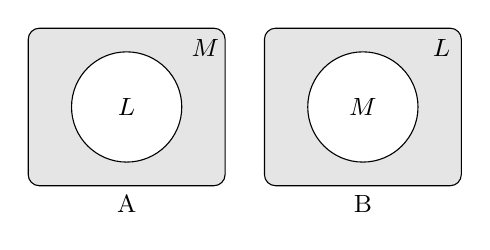
\begin{tikzpicture}[x=5mm, y=5mm,font=\small]
\definecolor{area}{gray}{0.9}
\draw [rounded corners, fill=area] (0,0) rectangle (5,4)  (4.5,3.5)node {$M$}; 
\draw[fill=white] (2.5,2) circle (1.4) node {$L$};
\node[below] at (2.5,0) {A};

\begin{scope}[xshift=30mm]
\draw [rounded corners, fill=area] (0,0) rectangle (5,4)  (4.5,3.5)node {$L$}; 
\draw[fill=white] (2.5,2) circle (1.4) node {$M$};
\node[below] at (2.5,0) {B};
\end{scope}
\end{tikzpicture}
\end{center}
\end{esercizio}

\begin{esercizio}
 \label{ese:10.11} %{ese:10.12}
 Attribuisci il valore di verità alle seguenti proposizioni:
\TabPositions{11.5cm}
\begin{enumeratea}
\item Il valore del monomio~$-a$ è negativo per qualunque $a$ diverso da zero.\tab\boxV\quad\boxF
\item Il valore del monomio~$-a^{2}$ è negativo per qualunque $a$ diverso da zero.\tab\boxV\quad\boxF
\item Il monomio~$b^{6}$ è il cubo di~$b^{2}$.\tab\boxV\quad\boxF
\item L'espressione~$ab^{-1}$ è un monomio.\tab\boxV\quad\boxF
\item Il valore del monomio $ab$ è nullo per~$a = 1$ e $b =-1$.\tab\boxV\quad\boxF
\end{enumeratea}
\end{esercizio}


\subsubsection*{10.3 - Moltiplicazione di due monomi}

\begin{esercizio}[\Ast]
 \label{ese:10.12} %{ese:10.13}
Determina il prodotto dei seguenti monomi.
\begin{multicols}{2}
\begin{enumeratea}
\spazielenx
 \item $\big(-x^{2}y^{4}\big)\cdot \bigg(-{\dfrac{8}{5}}x^{2}y\bigg)$;
 \item $\bigg(-{\dfrac{15}{28}}xy^{3}\bigg)\cdot\bigg(-\dfrac{7}{200}x^{2}y^{2}\bigg)$;
 \item $\big(a^{5}b^{5}y^{2}\big)\cdot\bigg(-\dfrac{8}{5}a^{2}y^{2}b^{3}\bigg)$;
 \item $\np{2,5}ab^{2}\cdot \bigg(-{\dfrac{1}{2}}a^{2}b\bigg)\cdot \np{1,5}a$;
 \item $\bigg(-{\dfrac{2}{9}}xz\bigg)\bigg(-{\dfrac{1}{4}}z^{3}\bigg)(27x)$;
 \item $-8\bigg(\dfrac{1}{4}x\bigg)\bigg(\dfrac{4}{5}x^{3}a^{4}\bigg)$;
 \item $5x^{3}y^{2}\cdot \bigg(-{\dfrac{1}{3}}x^{3}y^{2}\bigg)\cdot \bigg(-{\dfrac{1}{3}}\bigg)$;
 \item $6ab\cdot \bigg(-{\dfrac{1}{3}}a^{2}\bigg)\cdot {\dfrac{1}{2}ab\cdot 4a^{2}}$;
 \item $\bigg(\dfrac{7}{2}a^{3}x^{{4}}y^{2}\bigg)\cdot \bigg(-{\dfrac{8}{21}}ax^{2}y\bigg)$.
\end{enumeratea}
\end{multicols}
\end{esercizio}

%\pagebreak
\begin{esercizio}
 \label{ese:10.13} %{ese:10.14}
Determina il prodotto dei seguenti monomi.
\begin{multicols}{3}
\begin{enumeratea}
\spazielenx
 \item $(-2xy)\cdot (+3ax)$;
 \item $6a(-2ab)\big(-3a^{2}b^{2}\big)$;
 \item $(-1)(-ab)$;
 \item $\np{1,5}a^{2}b\cdot \bigg(-{\dfrac{2}{3}}a^{2}b\bigg)$;
 \item $-{\dfrac{7}{5}}xy^{3}\bigg(-{\dfrac{10}{3}}xy^{2}z\bigg)$;
 \item $-x\big(14x^{2}\big)$.
\end{enumeratea}
\end{multicols}
\end{esercizio}
\pagebreak
\begin{esercizio}[\Ast]
 \label{ese:10.14} %{ese:10.15}
Determina il prodotto delle seguenti coppie di monomi.
\begin{multicols}{3}
\begin{enumeratea}
 \item $\np{1,}\overline{{6}}xa\big(\np{1,2}xy^{2}\big)$;
 \item $\bigg(\dfrac{12}{7}m^{2}n^{3}\bigg)\bigg(-{\dfrac{7}{4}}mn\bigg)$;
 \item $\bigg(-{\dfrac{5}{4}}ax^{2}\bigg)\bigg(\dfrac{3}{10}x^{3}y\bigg)$;
 \item $12ab\bigg(-{\dfrac{1}{2}}a^{3}b^{3}\bigg)$;
 \item $\bigg(-{\dfrac{15}{8}}at^{2}\bigg)\bigg(\dfrac{6}{5}t^{3}x\bigg)$;
 \item $\bigg(\dfrac{12}{4}a^{2}n^{2}\bigg)\bigg(-{\dfrac{7}{4}}ax\bigg)$;
 \item $3ab^2\left(-2a^2b\right)\dfrac{ab}{2}$;
 \item $\dfrac{ab}{4}\left(-2x^2\right)(-2ax)$;
 \item $\dfrac{3}{5}a^4\left({2ab^2}\right)\left(-\dfrac{15}{6a^3b}\right)$.
\end{enumeratea}
\end{multicols}
\end{esercizio}


\begin{esercizio}
 \label{ese:10.15} %{ese:10.16}
In base agli esercizi precedenti puoi concludere che il grado del monomio prodotto è:

\begin{enumeratea}
 \item il prodotto dei gradi dei suoi fattori;
 \item la somma dei gradi dei suoi fattori;
 \item minore del grado di ciascuno dei suoi fattori;
 \item uguale al grado dei suoi fattori.
\end{enumeratea}
\end{esercizio}

\subsubsection*{10.4 - Potenza di un monomio}
\begin{esercizio}
 \label{ese:10.16} %{ese:10.17}
 Esegui le potenze indicate.
\begin{multicols}{2}
\begin{enumeratea}
\spazielenx
 \item $\bigg(-{\dfrac{3}{5}}abx^{3}y^{5}\bigg)^{3}=\dfrac{\ldots }{\ldots}a^{3}b^{3}x^{\ldots }y^{\ldots}$;
 \item $\big(-a^{4}b^{2}\big)^{7}=\ldots$;
 \item $\bigg(-3x^{3}y^{4}z\bigg)^{2}=9x^{6}y^{\ldots }z^{\ldots }$;
 \item $\bigg(\dfrac{1}{2}a^{2}bc^{5}\bigg)^{4}=\dfrac{1}{\ldots}a^{\ldots}b^{\ldots}c^{\ldots}$;
 \item $\big(a^{3}b^{2}\big)^{8}=\ldots$;
 \item $\big(-5ab^{2}c\big)^{3}=\ldots$
\end{enumeratea}
\end{multicols}
\end{esercizio}

\begin{esercizio}
 \label{ese:10.17} %{ese:10.18}
 Esegui le potenze indicate.
\begin{multicols}{3}
\begin{enumeratea}
\spazielenx
 \item $\big(+2ax^{3}y^{2}\big)^{2}$;
 \item $\bigg(-{\dfrac{1}{2}}axy^{2}\bigg)^{3}$;
 \item $\bigg(\dfrac{3}{4}x^{4}y\bigg)^{3}$;
 \item $\bigg(\dfrac{2}{3}xy^{2}\bigg)^{3}$;
 \item $\bigg(-{\dfrac{1}{2}}ab\bigg)^{4}$;
 \item $\bigg(-{\dfrac{3}{2}}a^{5}\bigg)^{2}$.
\end{enumeratea}
\end{multicols}
\end{esercizio}

\begin{esercizio}[\Ast]
 \label{ese:10.18} %{ese:10.19}
 Esegui le operazioni indicate.
\begin{multicols}{2}
\begin{enumeratea}
\spazielenx
 \item $\bigg[\big(-rs^{2}t\big)^{2}\bigg]^{3}$;
 \item $\Bigg[\bigg(-{\dfrac{1}{2}}x^{2}y^{3}\bigg)^{2}\Bigg]^{3}$;
 \item $\Bigg[\bigg(-{\dfrac{3}{2}}a^{2}b^{3}\bigg)^{2}\Bigg]^{2}$;
 \item $\big(-xy\big)^{2}\bigg(-{\dfrac{1}{2}}xy^{2}\bigg)^{3}$;
 \item $-\bigg(\dfrac{3}{2}xy^{2}\bigg)^{0}\cdot\bigg(-{\dfrac{1}{6}}xy\bigg)^{2}$;
 \item $-\bigg(-{\dfrac{1}{3}}x^{3}y^{2}\bigg)^{2}\cdot\bigg(-{\dfrac{1}{3}}\bigg)^{-3}$.
\end{enumeratea}
\end{multicols}
\end{esercizio}
\pagebreak
\begin{esercizio}[\Ast]
 \label{ese:10.19} %{ese:10.20}
 Esegui le operazioni indicate.
\begin{multicols}{2}
\begin{enumeratea}
\spazielenx
 \item $\bigg(\dfrac{2}{3}ab^{2}c\bigg)^{2}\cdot\big(-3ab^{3}\big)^{2}$;
 \item $\Bigg[\bigg(-{\dfrac{1}{2}}a^{2}b\bigg)^{2}\cdot{\dfrac{2}{3}a^{2}b}\Bigg]^{2}$;
 \item $\bigg(\dfrac{2}{3}x\cdot{\dfrac{1}{6}}x\cdot {\dfrac{1}{2}}x\bigg)^{2}\cdot\bigg(-{\dfrac{1}{6}}ab^{2}\bigg)^{2}$.
 \item $\left(-2x^2y^3\right)^2\left(2x^2y\right)^3$;
 \item $\left(-\dfrac{2}{5}xy^3\right)^3\left(\dfrac{5}{18}x^3y^5\right)^2\left(-3xy\right)^3$;
 \item $\left(-\dfrac{2}{3}xy^2\right)^2\left(-\dfrac{4}{9}a^2xy^3\right)^2\left(-\dfrac{3}{4}x^2\right)^3$.
\end{enumeratea}
\end{multicols}
\end{esercizio}

\subsubsection*{10.5 - Divisione di due monomi}
\begin{esercizio}[\Ast]
 \label{ese:10.20} %{ese:10.21}
Esegui le divisioni indicate e poni le condizioni di esistenza~$(\CE)$:
\begin{multicols}{2}
\begin{enumeratea}
\spazielenx
 \item $15b^{8}:\bigg(-{\dfrac{40}{3}}b^{3}\bigg)$;
 \item $\bigg(-{\dfrac{13}{72}}x^{2}y^{5}z^{3}\bigg):\bigg(-{\dfrac{26}{27}}xyz\bigg)$;
 \item $(-a^{7}):(8a^{7})$;
 \item $\bigg(\dfrac{1}{2}a^{3}\bigg):(-4a^{5})$;
 \item $\bigg(-{\dfrac{12}{2}}a^{7}b^{5}c^{2}\bigg):(-18ab^{4}c)$;
 \item $(-34x^{5}y^{2}):(-2yz^{3})$;
 \item $\dfrac{2}{5}a^3b^2:\left(-\dfrac{4}{5}ab^2c^2\right)$;
 \item $\dfrac{9}{5}a^4b^7c^2:\left(-\dfrac{3}{2}a^6b^5c\right)$.
% \item $\dfrac{2}{5}a^2b:\left(-\dfrac{3}{5}ab\right):\dfrac{5}{9}b$.
\end{enumeratea}
\end{multicols}
\end{esercizio}

\begin{esercizio}
 \label{ese:10.21} %{ese:10.22}
Esegui le divisioni indicate e poni le condizioni di esistenza~$(\CE)$:
\begin{multicols}{2}
\begin{enumeratea}
 \item $21a^{3}x^{4}b^{2}:7ax^{2}b$;
 \item $a^{6}:20a^{2}$;
 \item $20ax^{4}y:2xy$;
 \item $-72a^{4}b^{2}y^{2}:(-3ab^{2})$.
\end{enumeratea}
\end{multicols}
\end{esercizio}

\begin{esercizio}[\Ast]
 \label{ese:10.22} %{ese:10.23}
Esegui le divisioni indicate e poni le condizioni di esistenza~$(\CE)$:
\begin{multicols}{2}
\begin{enumeratea}
 \item $48a^{5}bx:a^{2}b$;
 \item $\Bigg[-\bigg(-{\dfrac{1}{3}}x^{3}y^{2}\bigg)^{2}:\bigg(-{\dfrac{1}{3}}\bigg)\Bigg]^{2}:(x^{3}y^{2})^{2}$;
 \item $\Bigg[\dfrac{3}{5}x^{4}:\bigg(\dfrac{1}{3}x^{4}\bigg)\Bigg]\cdot\Bigg[x^{4}:\bigg(\dfrac{4}{5}x^{4}\bigg)\Bigg]$;
 \item $\bigg(\dfrac{2}{3}ab^{2}c\bigg)^{2}:(-3ab^{3})$.
\end{enumeratea}
\end{multicols}
\end{esercizio}

\subsubsection*{10.6 - Addizione di due monomi simili}
\begin{esercizio}
 \label{ese:10.23} %{ese:10.24}
Determina la somma dei monomi simili~$8a^{2}b+(-{\frac{2}{3}})a^{2}b+\frac{1}{6}a^{2}b$.

La somma è un monomio \ldots\ldots\ldots agli
addendi; il suo coefficiente è dato da
$8-\frac{2}{3}+\frac{1}{6}=\ldots $, la parte letterale è~$\dotfill~$ Quindi la
somma è~$\dotfill$
\end{esercizio}

\begin{esercizio}
 \label{ese:10.24} %{ese:10.25}
Determina la somma~$2a-3ab-a+17ab+41a$.

I monomi addendi non sono tra loro simili, modifico la scrittura
dell'operazione applicando le proprietà associativa e commutativa
in modo da affiancare i monomi simili:
\[S=2a-3ab-a+17ab+41a=(\ldots\ldots\ldots)+(\ldots\ldots\ldots)=\ldots\ldots\ldots\]
La somma ottenuta non è un \ldots\ldots\ldots\ldots\ldots
\end{esercizio}
\pagebreak
\begin{esercizio}
 \label{ese:10.25} %{ese:10.26}
Esegui la somma algebrica dei seguenti monomi.
\begin{multicols}{3}
\begin{enumeratea}
 \item $6x+2x-3x$;
 \item $-3a+2a-5a$;
 \item $5a^{2}b-3a^{2}b$;
 \item $a^{2}b^{2}-3a^{2}b^{2}$;
 \item $2xy-3xy+xy$;
 \item $2y^{2}-3y^{2}+7y^{2}-4y^{2}$.
\end{enumeratea}
\end{multicols}
\end{esercizio}

\begin{esercizio}
 \label{ese:10.26} %{ese:10.27}
Esegui la somma algebrica dei seguenti monomi.
\begin{multicols}{3}
\begin{enumeratea}
 \item $-2xy^{2}+xy^{2}$;
 \item $-3ax-5ax$;
 \item $5ab-2ab$;
 \item $-3xy^{2}+3xy^{2}$;
 \item $7xy^{3}-2xy^{3}$;
 \item $+2xy^{2}-4xy^{2}$.
\end{enumeratea}
\end{multicols}
\end{esercizio}

\begin{esercizio}
 \label{ese:10.27} %{ese:10.28}
Esegui la somma algebrica dei seguenti monomi.
\begin{multicols}{2}
\begin{enumeratea}
 \item $\dfrac{1}{2}a^{2}-a^{2}$;
 \item $+2xy^{2}-4xy^{2}+xy^{2}$;
 \item $-5x^{2}+3x^{2}$;
 \item $\dfrac{1}{2}a+2a$;
 \item $5a^{2}b+2a^{2}b+a^{2}b-3a^{2}b-a^{2}b$;
 \item $\np{0,1}x-5x-\np{1,2}x+3x$.
\end{enumeratea}
\end{multicols}
\end{esercizio}

\begin{esercizio}[\Ast]
 \label{ese:10.28} %{ese:10.29}
Esegui la somma algebrica dei seguenti monomi.
\begin{multicols}{2}
\begin{enumeratea}
\spazielenx
 \item $\dfrac{1}{4}a^{3}b^{2}-\dfrac{1}{2}a^{3}b^{2}$;
 \item $\dfrac{2}{3}x-\dfrac{2}{5}x-2x+\dfrac{3}{10}x$;
 \item $\dfrac{2}{5}ab-\dfrac{1}{2}ab+\dfrac{27}{2}ab-\dfrac{1}{10}ab-\dfrac{5}{2}ab$;
 \item $-\bigg(-{\dfrac{1}{2}}ax^{2}\bigg)-3ax^{2}$;
 \item $-{\dfrac{9}{2}}xy-(-xy)$;
 \item $2xy^{2}-\dfrac{3}{2}xy^{2}-xy^{2}$.
\end{enumeratea}
\end{multicols}
\end{esercizio}

\begin{esercizio}[\Ast]
 \label{ese:10.29} %{ese:10.30}
Esegui la somma algebrica dei seguenti monomi.
\begin{multicols}{2}
\begin{enumeratea}
\spazielenx
 \item $\dfrac{1}{2}a+2a+(2a-a)-\bigg(3a-\dfrac{1}{2}a\bigg)$;
 \item $6xy^{2}+\dfrac{1}{3}xy^{2}-\dfrac{1}{4}xy^{2}-6xy^{2}$;
 \item $\dfrac{1}{2}xy^{2}+\dfrac{3}{2}xy^{2}$;
 \item $\bigg(\dfrac{2}{3}a+a\bigg)-\bigg(\dfrac{2}{3}a-a\bigg)$;
 \item $5ab-2ab+(-ab)-(+2ab)+ab$;
 \item $\np{-1,2}x^{2}+\np{0,1}x^{2}+(-5x)^{2}-(-25x)^{2}$.
\end{enumeratea}
\end{multicols}

\end{esercizio}


\begin{esercizio}[\Ast]
 \label{ese:10.30} %{ese:10.31}
Esegui le operazioni indicate.
\begin{multicols}{2}
\begin{enumeratea}
\spazielenx
 \item $6ab-\dfrac{1}{3}a^{2}+\dfrac{1}{2}ab+4a^{2}$;
 \item $\bigg(\dfrac{1}{4}x^{2}-\dfrac{3}{4}x^{2}+x^{2}\bigg)-\bigg(-{\dfrac{1}{3}}x^{2}+\dfrac{1}{2}x^{2}\bigg)$;
 \item $-{\dfrac{4}{3}}a^{2}b^{3}-2a^{2}b^{3}+\dfrac{1}{3}a^{2}b^{3}-a^{2}b^{3}$;
 \item $\big(-xy\big)^{2}\bigg(-{\dfrac{1}{2}}xy^{2}\bigg)+\dfrac{3}{2}xy^{2}\bigg(-{\dfrac{1}{6}}xy\bigg)^{2}$.
\end{enumeratea}
\end{multicols}
\end{esercizio}

\begin{esercizio}[\Ast]
 \label{ese:10.31} %{ese:10.32}
Esegui la somma algebrica dei seguenti monomi.

\begin{enumeratea}
\spazielenx
 \item $\dfrac{1}{2}x^{2}-2x^{2}-\bigg(-{\dfrac{1}{2}}x^{2}+\dfrac{3}{4}x^{2}-2x^{2}-\dfrac{3}{5}x^{2}\bigg)$;
 \item $5x^{3}y^{2}+\bigg(-{\dfrac{1}{3}}x^{3}y^{2}\bigg)+\bigg(-{\dfrac{1}{3}}\bigg)-\big(x^{3}y^{2}\big)+\bigg(-{\dfrac{1}{4}}x^{3}y^{2}\bigg)-\bigg(-{\dfrac{1}{3}}\bigg)$;
 \item $\bigg(2xy^{2}-\dfrac{3}{2}xy^{2}\bigg)-\big(xy^{2}+2xy^{2}-4xy^{2}\big)+\bigg(xy^{2}+\dfrac{1}{2}xy^{2}\bigg)$.
\end{enumeratea}
\end{esercizio}

\subsubsection*{10.7 - Espressioni con i monomi}
\begin{esercizio}[\Ast]
 \label{ese:10.32} %{ese:10.33}
Esegui le operazioni tra monomi.
\begin{multicols}{2}
\begin{enumeratea}
 \item $\bigg(-\dfrac{1}{2}a^{2}\bigg)\bigg(\dfrac{1}{2}a+2a\bigg)+a^{2}\bigg(3a-\dfrac{1}{2}a\bigg)$;
 \item $\bigg(\dfrac{2}{3}a-\dfrac{5}{2}a\bigg)a+\bigg(7a-\dfrac{1}{3}a\bigg)^{2}:2$;
 \item $\dfrac{1}{2}x^{2}\bigg(x^{2}+\dfrac{1}{2}x^{2}\bigg)-\dfrac{1}{6}x^{3}\bigg(12x-\dfrac{18}{5}x\bigg)$;
 \item $\bigg(-{\dfrac{3}{4}}x^{4}a^{2}b\bigg):\bigg(\dfrac{1}{2}x^{2}ab\bigg)+\dfrac{2}{3}x^{2}a$;
 \item $\bigg(\dfrac{1}{2}a-\dfrac{1}{4}a\bigg)^{2}:\bigg(\dfrac{3}{2}a-2a\bigg)$;
 \item $(3a-2a)(2x+2x):2a$.
\end{enumeratea}
\end{multicols}
\end{esercizio}

\begin{esercizio}[\Ast]
 \label{ese:10.33} %{ese:10.34}
Esegui le operazioni tra monomi.

\begin{enumeratea}
 \item $\bigg(\dfrac{1}{4}x^{2}-\dfrac{2}{3}x^{2}+x^{2}\bigg)\bigg(-{\dfrac{1}{3}}x+\dfrac{1}{2}x\bigg)$;
 \item $\bigg(\dfrac{1}{5}x-\dfrac{5}{2}x+x\bigg)-\bigg(2x-\dfrac{8}{3}x+\dfrac{1}{4}x+x\bigg)-\dfrac{7}{60}x$;
 \item $5a+\Bigg\{-{\dfrac{3}{4}}a-\bigg[2a-\dfrac{1}{2}a+\big(3a-a\big)+\np{0,5}a\bigg]-a\Bigg\}$;
 \item $-12x^{2}\bigg(\dfrac{1}{3}x\bigg)^{2}+\bigg[\np{0,1}x^{2}\big(-5x\big)^{2}-\big(-x^{2}\big)^{2}\bigg]$;
 \item $-{\dfrac{3}{5}}x^{2}y^{2}\bigg(-{\dfrac{10}{9}}xz^{2}\bigg)(-15xy)-\np{0,}\overline{{6}}x^{4}yz\big(\np{-0,}\overline{{7}}xy^{2}z\big)$;
 \item $\dfrac{1}{2}ab^{2}c+\Bigg[\dfrac{3}{4}a^{3}b^{6}c^{3}-\bigg(-{\dfrac{1}{4}ab^{2}c}\bigg)^{3}-\bigg(-{\dfrac{1}{2}ab^{2}}\bigg)^{2}\bigg(-{\dfrac{1}{16}ab^{2}c^{3}}\bigg)\Bigg]:%
 \bigg(-{\dfrac{5}{4}a^{2}b^{4}c^{2}}\bigg)$.
\end{enumeratea}
\end{esercizio}

\begin{esercizio}[\Ast]
 \label{ese:10.34} %{ese:10.35}
Esegui le operazioni tra monomi.

\begin{enumeratea}
 \item $\bigg(2xy^{2}-\dfrac{3}{2}xy^{2}\bigg)-\big(xy^{2}+2xy^{2}-4xy^{2}\big)+\bigg(xy^{2}+\dfrac{1}{2}xy^{2}\bigg)$;
 \item $\dfrac{1}{4}x^{4}y^{2}-\bigg[\dfrac{3}{2}x^{5}y^{4}:\bigg(\dfrac{1}{2}xy\bigg)^{2}-3x^{3}y^{2}\bigg]%
 \bigg(-{\dfrac{1}{3}}x\bigg)+\bigg(-{\dfrac{1}{2}}x^{2}y\bigg)^{2}$;
 \item $a^{2}-\Bigg\{a-\bigg[2\bigg(\dfrac{a}{2}-\dfrac{a}{3}\bigg)\bigg]\Bigg\}^{2}+%
 \bigg(\dfrac{2}{3}a+a\bigg)\bigg(\dfrac{2}{3}a-a\bigg)$;
 \item $\bigg[\bigg(-{\dfrac{1}{2}}a^{2}b\bigg)^{2}\cdot\bigg(-{\dfrac{2}{3}}b^{2}\bigg)^{2}-%
 \bigg(+{\dfrac{1}{3}}b^{3}a^{2}\bigg)^{2}\bigg]:\bigg(\dfrac{2}{3}a-\dfrac{1}{6}a+\dfrac{1}{2}a\bigg)+\bigg(-{\dfrac{1}{6}}ab^{2}\bigg)^2%
 \bigg(-{\dfrac{2}{5}}ab^2\bigg)$;
 \item $\left[\left(\dfrac{15}{4}x\right)^{2}:\left(\dfrac{4}{3}x+\dfrac{3}{4}x\right)\right]^{2}%
:(27x)+\left[\left(-{\dfrac{2}{3}}abx\right)^{2}-\left(\dfrac{1}{3}abx\right)^{2}\right]:(a^{2}b^{2}x)-x$;
 \item $x^{3}y^{3}-8x^{2}y^{2}(-2xy)-\dfrac{2}{5}x\left(-{\dfrac{5}{3}}x^{2}\right)\left(+3y^{3}\right)+\left(\dfrac{12}{7}xy^{2}\right)\left(-\dfrac{7}{4}x^{2}y\right)$.
\end{enumeratea}
\end{esercizio}


\begin{esercizio}[\Ast]
 \label{ese:10.35} %{ese:10.36}
Esegui le operazioni tra monomi.

\begin{enumeratea}
 \item $\dfrac{2}{3}a^{2}b-\bigg[3a-\dfrac{1}{3}a^{2}b-\bigg(\dfrac{2}{5}a+\dfrac{1}{2}a-3a\bigg)+\bigg(\dfrac{2}{5}a^{2}b+\dfrac{1}{2}a^{2}b-2a^{2}b\bigg)\bigg]%
 -\dfrac{1}{10}a^{2}b+\dfrac{51}{10}a$;
 \item $\bigg(\dfrac{1}{3}x+\dfrac{1}{2}x-2x\bigg)\bigg(-{\dfrac{1}{2}x^{2}}\bigg)+\bigg(\dfrac{3}{4}x^{2}-2x^{2}\bigg)\bigg(-{\dfrac{3}{5}x}\bigg)%
 -\dfrac{4}{3}\bigg(x^{3}+\dfrac{1}{2}x^{3}\bigg)$;
 \item 
 $\Bigg[-ab^{2}\cdot\bigg(-{\dfrac{3}{10}}+\dfrac{4}{5}-\dfrac{1}{2}\bigg)+\dfrac{10}{15}ab^{2}\Bigg]^{2}:\bigg[\bigg(b+\dfrac{3}{2}b\bigg)^{2}-\dfrac{5}{10}b^{2}+\dfrac{1}{2}b^{2}\bigg]\cdot\bigg(-{\dfrac{5}{2}ab}\bigg)^{2}$;
 \item $\bigg[\bigg(\dfrac{3}{2}xy\bigg)^{2}\cdot(\dfrac{4}{15}y\bigg)^{2}-\bigg(\dfrac{3}{2}xy^{2}\bigg)^{2}\cdot\bigg(\dfrac{2}{3}\bigg)^{3}%
 +\dfrac{8}{75}x^{2}y^{4}\bigg]:\bigg(\dfrac{10}{3}x^{2}y\bigg)$;
 \item $\bigg(\dfrac{1}{2}x+2x\bigg)\bigg(\dfrac{1}{2}x-2x\bigg)\bigg(\dfrac{1}{4}x^{2}-4x^{2}\bigg)-\dfrac{1}{4}x\bigg(\dfrac{27}{4}x^{3}-\dfrac{61}{3}x^{3}\bigg)%
 -16(x^{4}+x^{4})-\dfrac{1}{12}x^{2}\cdot x^{2}+\dfrac{1}{8}x^{4}$.
\end{enumeratea}
\end{esercizio}

\begin{esercizio}[\Ast]
 \label{ese:10.36} %{nuovo}
Esegui le operazioni tra monomi.

\begin{enumeratea}
 \item $\left[\left(-2a^2b\right)^3:\left(-6a^2\right)^2+\dfrac{1}{4}b(-ab)^2\right]^2:\left(\dfrac{1}{36}a^2b^3\right)$;
 \item $\left\lbrace 2x^2yz+\left[-\dfrac{3}{2}x^2yz-\left(-\dfrac{1}{2}x^2yz\right)\right] \right\rbrace:\left\lbrace-\left[-\left(-\dfrac{1}{2}x^2y\right)+\dfrac{1}{3}x^2y\right] \right\rbrace$;
 \item $\left(a^2\right)^3(-2a)^3-\left(\dfrac{1}{2}a^2\right)^3(-2a)^3+\left(\dfrac{3}{2}a^2\right)^4\left(-\dfrac{4}{9}a\right)$;
 \item $\left\lbrace-\left[-\left(-\dfrac{2}{3}x^4y^2-\dfrac{3}{2}x^4y^2\right)-2x^4y^2\right]\right\rbrace^2:\left[-2x^2y-\left(-\dfrac{1}{3}x^2y\right)\right]$;
 \item $\left\lbrace-\dfrac{1}{4}x^2\left[-x\left(-2y^2\right)^2:(-y)^4\right]^3 \right\rbrace^2:(-2x)^5+\dfrac{1}{2}x^2(-2x)^3$.
\end{enumeratea}
\end{esercizio}

\begin{esercizio}[\Ast]
 \label{ese:10.37} %{nuovo}
Esegui le operazioni tra monomi.

\begin{enumeratea}
 \item $\left(\dfrac{2}{3}abc^3:3c^2\right)-\left(\dfrac{2}{3}a^4b^5c^7:\dfrac{3}{5}a^3b^5c^7\right)$;
 \item $\left[\left(2ab^2c\right)^2:4a^2\right]-\left[\left(\dfrac{1}{4}a^3b^2c\right):\left(\dfrac{1}{2}a^3\right)^2\right]^3$;  \item $\left(a^2\right)^3(-2a)^3-\left(\dfrac{1}{2}a^2\right)^3(-2a)^3+\left(\dfrac{3}{2}a^2\right)^4\left(-\dfrac{4}{9}a\right)$;
 \item $\left(-4x^3y^7z^2\right)^2:\left(-4x^2y^4z\right)^3-xy^3\left(-2yz^2\right)^3:32xy^4z^5$;
 \item $6a^2b+\dfrac{8}{5}ab\cdot\dfrac{1}{2}a-3ab\cdot\dfrac{3}{4}a+\left(12a^3b^4:\dfrac{16}{3}ab^3\right)$.
\end{enumeratea}
\end{esercizio}

\begin{esercizio}
 \label{ese:10.38} %{ese:10.37}
Assegnati i monomi:
$m_{{1}}=\dfrac{3}{8}a^{2}b^{2}$, $m_{2}=-{\dfrac{8}{3}}ab^{3}$, $m_{3}=-3a$, $m_{{4}}=-{\dfrac{1}{2}}b$ e~$m_{{5}}=2b^{3}$.
Calcola il risultato delle seguenti operazioni, ponendo le opportune~$\CE$:
\begin{multicols}{3}
\begin{enumeratea}
 \item $m_{{1}}\cdot m_{2}\cdot (m_{{4}})^{2}$;
 \item $-m_{2}\cdot m_{{1}}\cdot (m_{3})^{2}\cdot m_{{5}}$;
 \item $(m_{3}\cdot m_{{4}})^{2}-m_{{1}}$;
 \item $m3\cdot m_{{5}}-m_{2}$;
 \item $m_{2}:m_{3}+m_{{5}}$;
 \item $m_{{1}}:m_{2}$.
\end{enumeratea}
\end{multicols}
\end{esercizio}

\begin{esercizio}
 \label{ese:10.39} %{ese:10.38}
Quando sottraiamo due monomi opposti otteniamo:
\begin{multicols}{2}
\begin{enumeratea}
\item il doppio del primo termine;
\item il doppio del secondo termine;
\item il monomio nullo;
\item 0.
\end{enumeratea}
\end{multicols}
\end{esercizio}
\pagebreak
\begin{esercizio}
 \label{ese:10.40} %{ese:10.39}
Quando dividiamo due monomi opposti otteniamo:
\begin{enumeratea}
\begin{multicols}{2}
\item~$-1$;
\item~0;
\item~1;
\item il quadrato del primo monomio.
\end{multicols}
\end{enumeratea}
\end{esercizio}

\begin{esercizio}
 \label{ese:10.41} %{ese:10.40}
Attribuisci il valore di verità alle seguenti proposizioni:
\TabPositions{11cm}
\begin{enumeratea}
 \item la somma di due monomi opposti è il monomio nullo \tab\boxV\quad\boxF
 \item il quoziente di due monomi simili è il quoziente dei loro coefficienti \tab\boxV\quad\boxF
 \item la somma di due monomi è un monomio \tab\boxV\quad\boxF
 \item il prodotto di due monomi è un monomio \tab\boxV\quad\boxF
 \item l'opposto di un monomio ha sempre il coefficiente negativo \tab\boxV\quad\boxF
\end{enumeratea}
\end{esercizio}

\begin{esercizio}[\Ast]
 \label{ese:10.42} %{ese:10.41}
Un quadrato è formato da~9~quadrati più piccoli, tutti di lato $ 2x $. Determina perimetro e area del quadrato.
\end{esercizio}

\begin{esercizio}[\Ast]
 \label{ese:10.43} %{ese:10.42}
Di un triangolo equilatero di lato $ a $ si raddoppiano due lati e si dimezza il terzo lato, si ottiene un triangolo \ldots\ldots\ldots Qual è la differenza tra i perimetri dei due triangoli?
\end{esercizio}

\subsubsection*{10.8 - Massimo Comune Divisore e minimo comune multiplo tra monomi}

\begin{esercizio}
 \label{ese:10.44} %{ese:10.43}
Vero o falso?

%\TabPositions{9cm}
\begin{multicols}{2}
\begin{enumeratea}
\item $12a^{3}b^{2}c$ è un multiplo di~$abc$; % \tab\boxV\quad\boxF
\item $2xy$ è un divisore di~$x^{2}$; % \tab\boxV\quad\boxF
\item $2a$ \ è divisore di~$4ab$; % \tab\boxV\quad\boxF
\item $-5b^{2}$ è divisore di~$15ab$; % \tab\boxV\quad\boxF
\item $8ab$ è multiplo di~$a^{2}b^{2}$; % \tab\boxV\quad\boxF
\item $12a^{5}b^{4}$ è multiplo di~$60a^{5}b^{7}$; % \tab\boxV\quad\boxF
\item $5$ è divisore di~$15a$. % \tab\boxV\quad\boxF
\end{enumeratea}
\end{multicols}
\end{esercizio}
%\pagebreak
\begin{esercizio}
 \label{ese:10.45} %{ese:10.44}
Vero o falso?

%\TabPositions{10cm}
\begin{enumeratea}
\item il~$\mcm$ fra monomi è divisibile per tutti i monomi dati; % \tab\boxV\quad\boxF
\item il~$\mcd$ fra monomi è multiplo di almeno un monomio dato; % \tab\boxV\quad\boxF
\item il~$\mcm$ è il prodotto dei monomi tra di loro. % \tab\boxV\quad\boxF
\end{enumeratea}
\end{esercizio}

\begin{esercizio}[\Ast]
 \label{ese:10.46} %{ese:10.45}
Calcola il~$\mcm$ e il~$\mcd$ dei seguenti gruppi di monomi.
\begin{multicols}{2}
\begin{enumeratea}
 \item $14x^{3}y^{2}$,\, $xy$,\, $4x^{3}y^{4}$;
 \item $xyz^{5}$,\,$x^{3}y^{2}z^{2}$;
 \item $4ab^{2}$,\, $a^{3}b^{2}$,\, $5ab^{5}$;
 \item $35x^4y^2z^3$,\, $42x^3y^2z$,\, $14x^2y^3z^2$.
\end{enumeratea}
\end{multicols}
\end{esercizio}

\begin{esercizio}
 \label{ese:10.47} %{ese:10.46}
Calcola il~$\mcm$ e il~$\mcd$ dei seguenti gruppi di monomi.
\begin{multicols}{2}
\begin{enumeratea}
 \item $2a^{2}bc^{3}$,\, $ab^{4}c^{2}$,\, $24a^{3}bc$;
 \item $6a^{2}x$,\, $2ax^{3}$,\, $4x^{2}c^{3}$;
 \item $30ab^{2}c^{4}$,\, $5a^{2}c^{3}$,\,$12abc$.
 \item $48xy^2z$,\, $36x^2yz$,\, $-24xyz^2$.
\end{enumeratea}
\end{multicols}
\end{esercizio}

\begin{esercizio}
 \label{ese:10.48} %{ese:10.47}
Calcola il~$\mcm$ e il~$\mcd$ dei seguenti gruppi di monomi.
\begin{multicols}{2}
\begin{enumeratea}
 \item $x^{2}y^{4}z^{2}$,\, $xz^{3}$,\, $24y^{2}z$;
 \item $4a^{2}y$,\, $y^{3}c$,\, $15ac^{5}$;
 \item $13xyc^{2}$,\, $x^{2}y^{3}c^{2}$\, $6c^{4}$.
 \item $\dfrac{1}{2}a^2bc^3$,\, $\dfrac{1}{4}a^{3}bc^{2}$,\, $\dfrac{3}{4}ab^4d$.
\end{enumeratea}
\end{multicols}
\end{esercizio}

\begin{esercizio}[\Ast]
 \label{ese:10.49} %{ese:10.48}
Calcola il~$\mcm$ e il~$\mcd$ dei seguenti gruppi di monomi.

\begin{enumeratea}
 \item $-2xy^{3}z$, $-6x^{3}yz$ e~$8x^{3}z$;
 \item $\frac{1}{4}ab^{2}c$, $-3a^{2}b^{2}c$ e~$-{\frac{1}{2}}ab^{2}c^{2}$;
 \item $\frac{2}{3}x^{2}y^{2}$, $\frac{1}{6}xy^{2}$ e~$\frac{2}{5}xyz^{2}$;
 \item $a^{n}b^{m}z^{2m+1}$, $a^{3n}b^{m+3}$ e~$a^{4n}b^{m+4}$.
\end{enumeratea}
\end{esercizio}

\begin{esercizio}
 \label{ese:10.50} %{ese:10.49}
Dati i monomi~$3xy^{2}$,\, $xz^{3}$

\begin{enumeratea}
\item calcola il loro~$\mcd$;
\item calcola il loro~$\mcm$;
\item verifica che il loro prodotto è uguale al prodotto tra il loro~$\mcm$ e il loro~$\mcd$;
\item verifica che il loro~$\mcd$ è uguale al quoziente tra il loro prodotto e il loro~$\mcm$.
\end{enumeratea}
\end{esercizio}

\subsection{Risposte}

\paragraph{10.12.} d)~$-\frac{15}{8}a^{2}b^{3}$,\quad f)~$-\frac{8}{5}x^{4}a^{4}$,\quad g)~$\frac{5}{9}x^{6}y^{4}$,\quad h)~$-4a^{6}b^{2}$,\quad i)~$-\frac{4}{3}a^{4}x^{6}y^{3}$.

\paragraph{10.14.} g)~$-3a^{4}b^{4}$,\quad h)~$a^{2}bx^{3}$,\quad i)~$-3a^{2}b$.

\paragraph{10.18.} b)~$\frac{1}{64}x^{12}y^{18}$,\quad e)~$\frac{1}{36}x^{2}y^{2}$.

\paragraph{10.19.} b)~$\frac{1}{36}a^{12}b^{6}$,\quad d)~$32x^{10}y^{9}$,\quad e)~$\dfrac{2}{15}x^{12}y^{22}$,\quad f)~$-\dfrac{1}{27}a^{4}x^{10}y^{10}$.

\paragraph{10.20.} b)~$\frac{3}{16}xy^{4}z^{2}$,\quad g)~$-\dfrac{a^2}{2c^2}$,\quad h)~$-\dfrac{6}{5}\dfrac{b^2c}{a^2}$.

\begin{multicols}{3}
\paragraph{10.22.} c)~$\frac{9}{4}$.
\paragraph{10.28.} c)~$\frac{54}{5}a^{3}b$.
\paragraph{10.29.} b)~$\frac{1}{12}xy^{2}$.
\paragraph{10.30.} d)~$-\frac{11}{24}x^{3}y^{4}$.
\paragraph{10.31.} c)~$3xy^{2}$.
\paragraph{10.32.} a)~$\frac{5}{4}a^{3}b$,\quad d)~$-\frac{5}{6}ax^{2}$.
\end{multicols}

\paragraph{10.33.} a)~$\frac{7}{72}x^{3}$,\quad b)~$-2x$, \quad c)~$-\frac{3}{4}a$, \quad d)~$\frac{1}{6}x^{4}$, \quad f)~$-\frac{1}{8}ab^{2}c$.

\paragraph{10.34.} a)~$3xy^{2}$,\quad b)~$\frac{3}{2}x^{4}y^{2}$, \quad c)~0, \quad d)~$-\frac{1}{90}a^{3}b^{6}$, \quad e)~$\frac{49}{48}x$, \quad f)~$16x^{3}y^{3}$.

\paragraph{10.35.} a)~$2a^{2}b$,\quad b)~$-\frac{2}{3}x^{3}$, \quad c)~$\frac{4}{9}a^{4}b^{4}$, \quad d)~$-\frac{3}{25}y^{3}$, \quad e)~$-\frac{29}{2}x^{4}$.

\paragraph{10.36.} a)~$-\frac{1}{36}a^{2}b^{3}$,\quad b)~$-\frac{6}{5}z$, \quad c)~$-\frac{37}{4}a^{9}$, \quad d)~$-\frac{1}{60}x^{6}y^{3}$, \quad e)~$-12x^{5}$.

\paragraph{10.42.} $24x$;\:$36x^2$.

\paragraph{10.43.} $\frac{3}{2}a$.

\paragraph{10.46.} a)~$28x^{3}y^{4};\:xy$,\quad b)~$x^{3}y^{2}z^{5};\:xyz^{2}$, \quad c)~$20a^{3}b^{5};\:ab^{2}$.

\paragraph{10.49.} a)~$a^{4n}b^{m+4}z^{2m+1};\:a^{n}b^{m}$,\quad b)~$24x^{3}y^{3}z;\:2xz$,\quad c)~$a^{2}b^{2}c^{2};\:ab^{2}c$,\quad d)~$x^{2}y^{2}z^{2};\:xy$.

\cleardoublepage
